% =============================================================================
% COPYRIGHT AND DISCLAIMER
% =============================================================================
% This file is provided as a convenience template for competition participants.
% By using it, you accept full responsibility for compliance with all applicable
% copyright, licensing, and usage rules of the Association for Computing
% Machinery (ACM) and of any LaTeX packages you load (including, without
% limitation, the "acmart" document class and related ACM materials).
%
% Consult ACM's official publication, template, and copyright policies before
% using this setup for any purpose other than this competition. Do not assume
% that this template may be reused, redistributed, or submitted elsewhere
% without independently verifying ACM's current rules.
%
% Use of the "acmart" class, the "sigconf" option, or ACM-style formatting in
% this template does NOT mean that this report, this competition, its organizers,
% or any resulting PDF is sponsored, endorsed, affiliated with, or published by
% ACM. ACM trademarks and branding remain the property of ACM.
%
% Template packages live in preamble.tex.
% Citations live in main.bib. Edit this file with your paper content.
% =============================================================================

\documentclass[sigconf]{acmart}
% =============================================================================
% Template setup — participants normally do not edit this file.
% Author content belongs in main.tex; citations belong in main.bib.
% \documentclass lives in main.tex so Overleaf does not treat this file as root.
% =============================================================================

% --- Competition / non-ACM-submission friendly rights metadata -------------
\setcopyright{none}
\settopmatter{printacmref=false}
\acmConference[Kaggle Competition]{Filament Segmentation Challenge}{2026}{\href{https://www.kaggle.com/competitions/filament-segmentation-2026}{kaggle.com/competitions/filament-segmentation-2026}}
\acmBooktitle{Competition Report}
\acmDOI{}
\acmISBN{}

% --- Author guidance text --------------------------------------------------
% \guide{...} is gray italic while \guideStyletrue; omitted from the PDF if false.
% Flip the switch in main.tex after % =============================================================================
% Template setup — participants normally do not edit this file.
% Author content belongs in main.tex; citations belong in main.bib.
% \documentclass lives in main.tex so Overleaf does not treat this file as root.
% =============================================================================

% --- Competition / non-ACM-submission friendly rights metadata -------------
\setcopyright{none}
\settopmatter{printacmref=false}
\acmConference[Kaggle Competition]{Filament Segmentation Challenge}{2026}{\href{https://www.kaggle.com/competitions/filament-segmentation-2026}{kaggle.com/competitions/filament-segmentation-2026}}
\acmBooktitle{Competition Report}
\acmDOI{}
\acmISBN{}

% --- Author guidance text --------------------------------------------------
% \guide{...} is gray italic while \guideStyletrue; omitted from the PDF if false.
% Flip the switch in main.tex after % =============================================================================
% Template setup — participants normally do not edit this file.
% Author content belongs in main.tex; citations belong in main.bib.
% \documentclass lives in main.tex so Overleaf does not treat this file as root.
% =============================================================================

% --- Competition / non-ACM-submission friendly rights metadata -------------
\setcopyright{none}
\settopmatter{printacmref=false}
\acmConference[Kaggle Competition]{Filament Segmentation Challenge}{2026}{\href{https://www.kaggle.com/competitions/filament-segmentation-2026}{kaggle.com/competitions/filament-segmentation-2026}}
\acmBooktitle{Competition Report}
\acmDOI{}
\acmISBN{}

% --- Author guidance text --------------------------------------------------
% \guide{...} is gray italic while \guideStyletrue; omitted from the PDF if false.
% Flip the switch in main.tex after \input{preamble}.
%
% Do not use \guide{...} for \email{...}.
\usepackage{xcolor}
\newif\ifguideStyle
\guideStyletrue
\newcommand{\guide}[1]{%
  \ifguideStyle
    {\color{gray!65}\itshape #1}%
  \fi
}

% --- Math ------------------------------------------------------------------
% Do NOT load amssymb (or amsfonts): acmart already loads newtxmath, which
% defines the same symbols (e.g. \Bbbk) and causes a conflict on Overleaf.
% amsmath is already provided by acmart; mathtools extends it.
\usepackage{mathtools}

% --- Figures ---------------------------------------------------------------
% graphicx is already loaded by acmart
\usepackage{subcaption}

% --- Tables ----------------------------------------------------------------
% booktabs is already loaded by acmart
\usepackage{tabularx}
\usepackage{multirow}

% --- Bibliography style is set in main.tex (ACM-Reference-Format) ----------
.
%
% Do not use \guide{...} for \email{...}.
\usepackage{xcolor}
\newif\ifguideStyle
\guideStyletrue
\newcommand{\guide}[1]{%
  \ifguideStyle
    {\color{gray!65}\itshape #1}%
  \fi
}

% --- Math ------------------------------------------------------------------
% Do NOT load amssymb (or amsfonts): acmart already loads newtxmath, which
% defines the same symbols (e.g. \Bbbk) and causes a conflict on Overleaf.
% amsmath is already provided by acmart; mathtools extends it.
\usepackage{mathtools}

% --- Figures ---------------------------------------------------------------
% graphicx is already loaded by acmart
\usepackage{subcaption}

% --- Tables ----------------------------------------------------------------
% booktabs is already loaded by acmart
\usepackage{tabularx}
\usepackage{multirow}

% --- Bibliography style is set in main.tex (ACM-Reference-Format) ----------
.
%
% Do not use \guide{...} for \email{...}.
\usepackage{xcolor}
\newif\ifguideStyle
\guideStyletrue
\newcommand{\guide}[1]{%
  \ifguideStyle
    {\color{gray!65}\itshape #1}%
  \fi
}

% --- Math ------------------------------------------------------------------
% Do NOT load amssymb (or amsfonts): acmart already loads newtxmath, which
% defines the same symbols (e.g. \Bbbk) and causes a conflict on Overleaf.
% amsmath is already provided by acmart; mathtools extends it.
\usepackage{mathtools}

% --- Figures ---------------------------------------------------------------
% graphicx is already loaded by acmart
\usepackage{subcaption}

% --- Tables ----------------------------------------------------------------
% booktabs is already loaded by acmart
\usepackage{tabularx}
\usepackage{multirow}

% --- Bibliography style is set in main.tex (ACM-Reference-Format) ----------

\usepackage{tikz}  % Fig. 1 (figures/pipeline.tex)
\usetikzlibrary{arrows.meta}
\setlength{\emergencystretch}{1.5em}  % lets TeX reflow a line instead of overflowing into the margin

% Guide styling: \guideStyletrue = show gray italic hints; \guideStylefalse = omit them
% Off for submission: every \guide{} placeholder is filled.
% \guideStyletrue
\guideStylefalse

% Template text: \tpl{} wraps the text that is black in the original template (not to be altered).
% \templateRedtrue = show it in red, to check it is unchanged; switch to \templateRedfalse before submitting.
\newif\iftemplateRed
% \templateRedtrue
\templateRedfalse
\NewDocumentCommand{\tpl}{+m}{\leavevmode{\iftemplateRed\color{red}\fi#1}}

% Latest changes: \chg{} wraps the text changed in the latest revision (green while \showChangestrue).
% Marks are cleared at the next revision; switch to \showChangesfalse (or remove the marks) before submitting.
\newif\ifshowChanges
% \showChangestrue
\showChangesfalse
\NewDocumentCommand{\chg}{+m}{\leavevmode{\ifshowChanges\color{green!55!black}\fi#1}}

\begin{document}

\title[A Learned Candidate Scorer for Solar Filament Segmentation]{A Learned Candidate Scorer over Two Mask2Former Families for Solar Filament Instance Segmentation}  % [short title]: running head of odd pages, which the full title overlapped
\subtitle{\tpl{A Solution to the Solar Filament Segmentation Challenge 2026}} % DO NOT CHANGE

% Last revision from GP (me)
\newif\ifshowGp
\showGpfalse       % switch to \showGpfalse to print the text in black
\NewDocumentCommand{\gp}{+m}{\leavevmode{\ifshowGp\color{blue}\fi#1}}

\author{Guillaume PELLUET}
\orcid{0000-0002-6537-6768}
\affiliation{%
  \country{France}
}
\email{gpelluet@gmail.com}

\begin{abstract}
    % Context
    \tpl{This report describes our solution to the Solar Filament Segmentation Challenge~2026, a Kaggle competition on automatic segmentation of solar filaments in GONG H-$\alpha$ observations.} Filaments are thin, elongated and of very different sizes, must be told apart from other dark features such as sunspots, and are annotated inconsistently: two annotators of the same photograph agree at a panoptic quality (PQ) of only 0.340. 
    % Method
    \gp{Given this low agreement and the difficulty of segmenting thin objects, we split the problem into three stages. (i)~\textit{Candidate generation}: two Mask2Former families propose candidate filaments. (ii)~\textit{Scoring}: a gradient-boosted model, fed by independently trained evidence models, predicts the IoU each candidate will reach with the annotators, and the non-overlapping set that maximises the expected PQ is kept. (iii)~\textit{Refinement}: the boundary of each kept mask is redrawn from full-resolution U-Net maps, to follow the edges and barbs of the filament.}
    % Perfs.
    Out of fold on the 707 training observations, the pipeline reaches a PQ of \textbf{0.4801} (95\% interval 0.4714--0.4882), against 0.4629 for one Mask2Former with a fixed threshold; it scores \textbf{0.42} on the public and \chg{\textbf{0.39} on the private leaderboard.}

\end{abstract}

\maketitle

\ifguideStyle
\noindent{\color{gray!65}\itshape
Guide mode is on.}
\par\medskip
\fi


% ==================================== %
%              INTRODUCTION            %
% ==================================== %
\section{\texorpdfstring{\tpl{Introduction}}{Introduction}}
    \tpl{This report goes over the details of our submitted solution to the Solar Filament Segmentation Challenge~2026 \cite{filament-segmentation-2026}. The challenge, launched on July~10,~2026, is organized by the Earth-Space AI Research (ESAIR) Lab\footnote{\href{https://www.esairlab.com/home}{www.esairlab.com/}}. This challenge utilizes the MAGFiLO dataset for evaluation of the segmentation algorithms \cite{ahmadzadeh2024dataset}.} We address it as instance segmentation of the filaments, scored by panoptic quality (PQ)~\cite{kirillov2019panoptic}.

    Two observations shaped our solution. First, our first model already finds most filaments: among the masks it proposes on 8 rotated and flipped views of a photograph, 85--89\% of the annotated filaments have a matching mask. A fixed score threshold, however, keeps the matching mask for only about two thirds of them. The bottleneck is therefore choosing which masks to submit, not generating them. Second, the annotations are noisy: two annotators of the same image agree at a PQ of only 0.340. 
    We therefore spent most of our effort on choosing which candidates to submit, with a scorer trained on the exact question the metric asks, and checked every step on out-of-fold PQ with paired bootstrap intervals. Our code, the trained models and a notebook that reproduces the submission are public\footnote{\href{https://github.com/Emualliug2705/kaggle_filament_2026}{github.com/Emualliug2705/kaggle\_filament\_2026}}.


% ==================================== %
%              METHODOLOGY             %
% ==================================== %
\section{\texorpdfstring{\tpl{Methodology}}{Methodology}}\label{sec:methodology}

\begin{figure*}[t]
\centering
% Fig. 1: the pipeline in four parts (TikZ; replaces pipeline.png / pipeline.drawio).
% Parts and colours: 1 Data (gray), 2 Candidate generation (blue), 3 Selection (orange), 4 Refinement (green).
% Input from main.tex inside a figure*; needs \usepackage{tikz} and \usetikzlibrary{arrows.meta}.
\definecolor{pdata}{HTML}{52514E}\definecolor{pdataF}{HTML}{E9E9E9}
\definecolor{pcand}{HTML}{2A78D6}\definecolor{pcandF}{HTML}{E5EEFA}
\definecolor{psel}{HTML}{EB6834}\definecolor{pselF}{HTML}{FCECE6}
\definecolor{pref}{HTML}{1BAF7A}\definecolor{prefF}{HTML}{E3F5EE}
\definecolor{parrow}{HTML}{4A4A4A}
\begin{tikzpicture}[
    x=1cm, y=1cm,
    font=\scriptsize\sffamily,
    box/.style={draw, rounded corners=3pt, line width=0.8pt, align=center, inner sep=2.5pt, text width=#1},
    box/.default=2.3cm,
    data/.style={box=#1, draw=pdata, fill=pdataF}, data/.default=1.95cm,
    cand/.style={box=#1, draw=pcand, fill=pcandF}, cand/.default=2.3cm,
    sel/.style={box=#1, draw=psel, fill=pselF}, sel/.default=2.4cm,
    ref/.style={box=#1, draw=pref, fill=prefF}, ref/.default=2.45cm,
    flow/.style={-{Stealth[length=4pt]}, line width=0.6pt, draw=parrow},
    part/.style={draw=#1, dashed, rounded corners=5pt, line width=0.5pt, fill=#1!4},
    head/.style={font=\footnotesize\sffamily\bfseries, text=#1, anchor=north},
  ]
  % ---- part frames and headers -------------------------------------------------------------------
  \def\ybot{-0.75} \def\ytop{5.35}
  \path[part=pdata] (0.00,\ybot) rectangle (2.35,\ytop);
  \path[part=pcand] (2.55,\ybot) rectangle (8.05,\ytop);
  \path[part=psel]  (8.25,\ybot) rectangle (14.35,\ytop);
  \path[part=pref]  (14.55,\ybot) rectangle (17.55,\ytop);
  \node[head=pdata] at (1.175,\ytop-0.08) {1.\enspace Data};
  \node[head=pcand] at (5.30,\ytop-0.08)  {2.\enspace Candidate generation};
  \node[head=psel]  at (11.30,\ytop-0.08) {3.\enspace Selection};
  \node[head=pref]  at (16.05,\ytop-0.08) {4.\enspace Refinement};

  % ---- 1 Data --------------------------------------------------------------------------------------
  \node[data] (photo) at (1.175,2.45) {H-$\alpha$ photograph\\2048$\times$2048\\[3pt]707 training,\\5 folds grouped\\by day};

  % ---- 2 Candidate generation ---------------------------------------------------------------------
  \node[cand] (m2fg) at (3.95,3.75) {Mask2Former,\\grayscale\\5 folds $\times$ 8 views};
  \node[cand] (m2fl) at (3.95,1.55) {Mask2Former,\\limb-corrected\\5 folds $\times$ 8 views};
  \node[cand=1.95cm] (fuse) at (6.85,2.65) {fuse the 16 views\\(IoU link 0.5,\\pixel vote)\\$=$ candidate pool};

  % ---- 3 Selection --------------------------------------------------------------------------------
  \node[sel] (feat) at (9.80,3.70) {129 numbers per\\candidate: shape,\\scores, contrast,\\agreement with\\evidence models};
  \node[sel] (evid) at (9.80,1.00) {evidence models\\(5 folds each):\\Mask R-CNN, 3 U-Nets\\(probability, spine),\\tiled detector};
  \node[sel] (scor) at (12.85,4.10) {LightGBM scorer\\$q$ = expected\\matched IoU};
  \node[sel] (selx) at (12.85,2.62) {exact selection\\max $\sum(q-\tau)$,\\overlap $<\theta$};
  \node[sel] (test) at (12.85,1.02) {on test: candidates\\of the 5 fold models\\fused, then selected\\with the OOF $\tau$, $\theta$};

  % ---- 4 Refinement -------------------------------------------------------------------------------
  \node[ref] (redr) at (16.05,2.62) {boundary redrawn\\within 2 px from\\the U-Net maps\\[2pt]$\rightarrow$ submission};

  % ---- arrows -------------------------------------------------------------------------------------
  \draw[flow] (photo.east) -- (m2fg.west);
  \draw[flow] (photo.east) -- (m2fl.west);
  \draw[flow] (photo.south) -- (1.175,-0.25) -- (8.15,-0.25) |- (evid.west);
  \draw[flow] (m2fg.east) -- (fuse.west);
  \draw[flow] (m2fl.east) -- (fuse.west);
  \draw[flow] (fuse.east) -- (feat.west);
  \draw[flow] (evid.north) -- (feat.south);
  \draw[flow] (feat.east) -- (scor.west);
  \draw[flow] (scor.south) -- (selx.north);
  \draw[flow] (selx.south) -- (test.north) node[midway, right=1pt, font=\tiny\sffamily] {$\tau$, $\theta$};
  \draw[flow] (test.east) -- (redr.west);
  \draw[flow, dashed] (evid.south) -- (9.80,-0.25) -- (16.05,-0.25) node[pos=0.5, below=0pt, font=\tiny\sffamily\itshape, text=parrow] {U-Net maps} -- (redr.south);
\end{tikzpicture}

\caption{The pipeline, in four parts: (1)~data, (2)~candidate generation, (3)~selection and (4)~refinement, described in Sections~\ref{sec:data} to~\ref{sec:refinement}. Every model family is trained 5 times, once per fold. On a training photograph, every number comes from models that did not train on its fold; on a test photograph, the candidates of the 5 fold models are fused before the selection.}
\label{fig:pipeline}
\Description{Flow chart in four parts. Data: the photograph and the 5 folds. Candidate generation: two Mask2Former families whose 16 views are fused into a candidate pool. Selection: evidence models give 129 numbers per candidate to a LightGBM scorer, followed by an exact selection; on test, the candidates of the 5 fold models are fused before that selection. Refinement: the boundary of each kept mask is redrawn from the U-Net maps, giving the submission.}
\end{figure*}

\subsection{\texorpdfstring{\chg{Data, preprocessing}}{Data, preprocessing} and folds}\label{sec:data}
The training set has 707 GONG \cite{harvey1996gong} observations with one to three annotators each, giving 1,154 annotator records and 8,199 filaments. They were taken on 656 days, and photographs of the same day show the same filaments. We therefore draw 5 folds as a group k-fold over the observation day: no day is shared between folds, and every fold holds photographs from at least 11 of the 12 years and all six sites. Every model family is trained 5 times, model $k$ on the other four folds, so its predictions on fold $k$ are out of fold (OOF); the scorer is cross-fitted on the same folds.

\chg{Each observation is a $2048 \times 2048$ 8-bit grayscale JPEG. As a filament can be only a few pixels wide, every model reads it at native resolution, as crops, tiles or whole photographs, except the box refiner, which resamples its context crop to 512 pixels. The annotated polygons are rasterised into one binary mask per filament and per annotator record, and one training sample is one record. For Mask2Former, the photograph is replicated to three channels, scaled to $[0, 1]$ and standardised with the ImageNet statistics of the COCO weights. For the U-Nets, it is standardised by the mean and standard deviation of its own solar disk, which removes most brightness differences between sites and dates, and clipped.}

\subsection{Candidate generation: two Mask2Former families}\label{sec:candidates}
\chg{\paragraph{\textbf{Architecture}} Mask2Former \cite{cheng2022mask2former} predicts a set of masks, each with a class. (i)~A Swin-S backbone \cite{liu2021swin}, a hierarchical transformer with shifted-window attention, extracts features at 1/4 to 1/32 of the input resolution. (ii)~A pixel decoder of six multi-scale deformable-attention layers fuses them into a per-pixel embedding at 1/4 resolution. (iii)~A transformer decoder refines 100 learned queries over nine layers, each attending to one scale in turn, with masked attention: a query only attends to the pixels of the mask it predicted at the previous layer. Each query gives a class probability (filament or no object) and an embedding whose dot product with the per-pixel embeddings gives its mask logits. In training, queries are matched one-to-one to the annotated filaments by the Hungarian algorithm~\cite{kuhn1955hungarian}, and the loss, summed over the predictions of every decoder layer $\ell$, is
\begin{equation}
  \begin{aligned}
    \mathcal{L} &= \textstyle\sum_{\ell} \big( 2\,\mathcal{L}^{\ell}_{\mathrm{cls}} + 5\,\mathcal{L}^{\ell}_{\mathrm{BCE}} + 5\,\mathcal{L}^{\ell}_{\mathrm{Dice}} \big), \\
    \mathcal{L}_{\mathrm{cls}} &= -\frac{\sum_{i} w_i \log p_i(c_i)}{\sum_{i} w_i}, \quad w_i = \begin{cases} 1 & \text{matched} \\[-2pt] 0.1 & \text{else} \end{cases}
  \end{aligned}
  \label{eq:m2f}
\end{equation}
where $p_i(c_i)$ is the probability query $i$ gives its target class (filament if matched, no object otherwise), and the BCE and Dice terms compare each matched mask with its filament. These are the reference settings; only the COCO classifier is replaced, by one filament class.}

\paragraph{\textbf{Training}} Both families start from the COCO \cite{lin2014coco} instance segmentation weights and are trained with AdamW and a cosine decay, with a lower learning rate for the backbone. A step holds either native-resolution crops or whole photographs, accumulated one sample at a time to fit in GPU memory. Crops are centred on a random filament; samples are flipped, rotated by multiples of $90^\circ$ and changed in gamma and gain. The first family reads the grayscale photograph. The second reads three channels: the photograph, the disk divided by its radial median profile (a limb-darkening correction; the disk is found by a Hough circle) and a CLAHE copy of it, with randomly zoomed crops.

\paragraph{\textbf{Inference and view fusion}} Mask logits come out at 1/4 resolution (512 pixels) and are upsampled bilinearly to 2048 pixels and thresholded at 0.5. Every mask whose class probability and area exceed small floors becomes a candidate, scored by its class probability times its mean mask probability. Each fold model predicts the 8 rotations and reflections, and the 16 views of a fold's two models are fused: in decreasing score, each ungrouped candidate starts a group and takes every ungrouped candidate whose IoU with it exceeds a link threshold; a pixel belongs to the group's mask if half of its $m$ members cover it, and the group's score is the mean member score times $(0.5 + 0.5\,m/16)$.

\subsection{Scoring and selection}\label{sec:selection}
\paragraph{\textbf{Evidence models}} Three kinds of evidence models (six networks, each trained on the same folds) check each candidate independently.
(i)~A Mask R-CNN \cite{he2017maskrcnn} (ResNet-50 FPN v2) proposes its own instances\chg{: region proposals on a feature pyramid, each refined into a box, a score and a mask}. 
(ii)~Three U-Nets \cite{ronneberger2015unet}\chg{, encoder--decoders,} with ConvNeXt-T \cite{liu2022convnext} (two) and ResNet-34 \cite{he2016resnet} encoders, predict two full-resolution maps: the filament probability (target: the fraction of annotators who marked the pixel) and the filament spine (its centre line), with BCE and Dice losses. 
(iii)~A tiled Faster R-CNN \cite{ren2015faster} proposes boxes on 9 overlapping tiles, and a ResNet-18 U-Net draws the mask inside each box.

\paragraph{\textbf{A scorer trained on the metric's question}} For each candidate of a training observation, the target is the mean over its annotator records of the IoU with the annotated filament it overlaps most, counted as zero when not above 0.5: exactly what the candidate adds to the PQ numerator. The scorer reads 129 numbers per candidate: 30 on the candidate itself (fused score, area, elongation, position on the disk, contrast, overlapping competitors), 10 on its agreement with the Mask R-CNN and tiled-detector instances, 72 on the spine and probability maps of the three U-Nets inside and around it, and 17 on how stable it is across the 16 raw views. LightGBM \cite{ke2017lightgbm}\chg{, gradient-boosted regression trees, each fitted to the errors of the previous ones}, is averaged over several random seeds. Its OOF predictions correlate with the target at 0.780, against 0.702 for the fused score.

\paragraph{\textbf{Exact selection}} PQ \cite{kirillov2019panoptic} is
\begin{equation}
  \mathrm{PQ} = \frac{\sum_{(\hat{y}, y) \in \mathrm{TP}} \mathrm{IoU}(\hat{y}, y)}{|\mathrm{TP}| + \tfrac12 |\mathrm{FP}| + \tfrac12 |\mathrm{FN}|},
  \label{eq:pq}
\end{equation}
so a mask raises the score only if its expected matched IoU exceeds PQ/2. Among the $n$ candidates of a photograph, with masks $M_i$ and predictions $q_i$, we keep the set $\{i : x_i = 1\}$ solving
\begin{equation}
  \begin{aligned}
    \max_{x \in \{0,1\}^n}\ & \textstyle\sum_{i} x_i\,(q_i - \tau) \\
    \text{s.t.}\ & x_i + x_j \le 1 \ \text{ if } \frac{|M_i \cap M_j|}{\min(|M_i|, |M_j|)} > \theta,
  \end{aligned}
  \label{eq:select}
\end{equation}
that is, the set with the largest total expected gain in which no two masks overlap by more than a fraction $\theta$ of the smaller one. It is solved exactly, per connected component of the conflict graph, as a 0/1 integer program with HiGHS \cite{huangfu2018highs}. Unlike greedy non-maximum suppression, this can prefer two halves of a filament to one whole mask conflicting with both. The kept masks are painted in decreasing $q$, so that each pixel goes to one mask. $\theta$ and $\tau$ are chosen on OOF PQ (Section~\ref{sec:details}), and $\tau$ comes out close to PQ/2, as expected. On test, the scorer is retrained on all OOF rows, the candidates of the 5 fold models are fused as the views are, and a group's $q$ is the mean over the 5 models of that model's best member.

\subsection{Refinement: boundary redraw}\label{sec:refinement}
Mask2Former's masks come from quarter-resolution logits, while the U-Nets predict at full resolution. So Mask2Former decides where the filament is and roughly how big it is. Each kept mask $M$ keeps its extent, and its boundary is redrawn within $r$ pixels from $P$, the mean probability map of two U-Nets, shifted by a fraction of a pixel upwards, where the annotators' outlines sit on average from our analysis. With $C = \mathrm{erode}(M, r)$ and $O = \mathrm{dilate}(M, r)$, the new mask is $C$ plus the pixels of $O \setminus C$ with the highest $P$, up to the geometric mean of $|M|$ and of the U-Net area $|C \cup ((P > 0.5) \cap O)|$. The redrawn masks are painted again in decreasing $q$, masks below a minimum area are dropped, and each remaining mask is written to the submission as a COCO run-length encoding.


% ==================================== %
%              EVALUATION              %
% ==================================== %
\section{\texorpdfstring{\tpl{Evaluation}}{Evaluation}}\label{sec:evaluation}

\begin{table}[t]
\centering
\small
\caption{OOF PQ on the 707 training observations, adding one step at a time. $\Delta$: paired difference with the row above, with its 95\% bootstrap interval. $\dagger$:~against a rerun of the row above with $\tau$ chosen on all folds (0.4744).}
\label{tab:results}
\newcommand*{\twoline}[2]{\begin{tabular}{@{}c@{}}#1\\ #2\end{tabular}}
\renewcommand{\tabularxcolumn}[1]{m{#1}}
\setlength{\tabcolsep}{4pt}
\begin{tabularx}{\columnwidth}{@{}>{\raggedright\arraybackslash}Xcc@{}}
\toprule
Step & OOF PQ & \twoline{$\Delta$}{{[}95\% interval{]}} \\
\midrule
Grayscale family, single view, score~$>0.85$ & 0.4629 & -- \\
Two families, 16-view pool, score $>0.75$ & 0.4693 & -- \\
+ learned scorer, exact selection (nested~$\tau$) & 0.4739 & \textbf{\boldmath\twoline{$+0.0046$}{{[}$+0.0014$, $+0.0076${]}}} \\
+ boundary redraw, $r=2$~$\dagger$ & 0.4783 & \twoline{$+0.0039$}{{[}$+0.0025$, $+0.0054${]}} \\
+ view stability, U-Net probability, 10 seeds & \textbf{0.4801} & \twoline{$+0.0018$}{{[}$-0.0004$, $+0.0039${]}} \\
\midrule
Same pipeline, grayscale family only & -- & \twoline{$-0.0004$}{{[}$-0.0028$, $+0.0020${]}} \\
\bottomrule
\end{tabularx}
\end{table}

\subsection{Protocol and results}
\paragraph{\textbf{Protocol}} All numbers are OOF PQ over the 707 training observations, computed as in the competition: each annotator record is matched separately and the counts are pooled before PQ is computed once. All parameters were tuned on this OOF PQ; a difference is judged with a paired bootstrap over observations (4,000 resamples), and $\tau$ is also chosen on 4 folds and applied to the fifth (nested) to check that it is not overfitted. Semantic models (a basic CNN, U-Net, UNet~3+ \cite{huang2020unet3plus}) scored lower than Mask2Former, which predicts each filament as its own mask, as PQ requires, instead of splitting a map into connected components.

\paragraph{\textbf{Results}} Tab.~\ref{tab:results} adds one step at a time to decompose our approach. \gp{Fusing the 16 views and learning the scorer bring the largest gains. The scorer needs the evidence models: on the candidate's own numbers it does no better than a fixed threshold, the U-Net spine maps bring most of its gain. With a pool that already holds a candidate for 85--89\% of the filaments, this shows that the difficulty of this challenge lies more in choosing which candidates to submit than in segmenting them.}
The final pipeline scores \textbf{0.4801} (95\% interval 0.4714--0.4882), well above the 0.340 at which two annotators agree; its folds range from 0.4733 to 0.4909, so differences below about 0.005 between single rows are noise. Of its 7,378 masks, 5,409 match one of the 8,199 annotated filaments, with a mean IoU of 0.691. 
Regarding the test and so the leaderboard of the competition, the final submission scores \textbf{0.42} on the public leaderboard \chg{and \textbf{0.39} on the private one}, \gp{ranking 36th and 10th of 1,708 teams, respectively}.

\begin{figure*}[t]
\centering
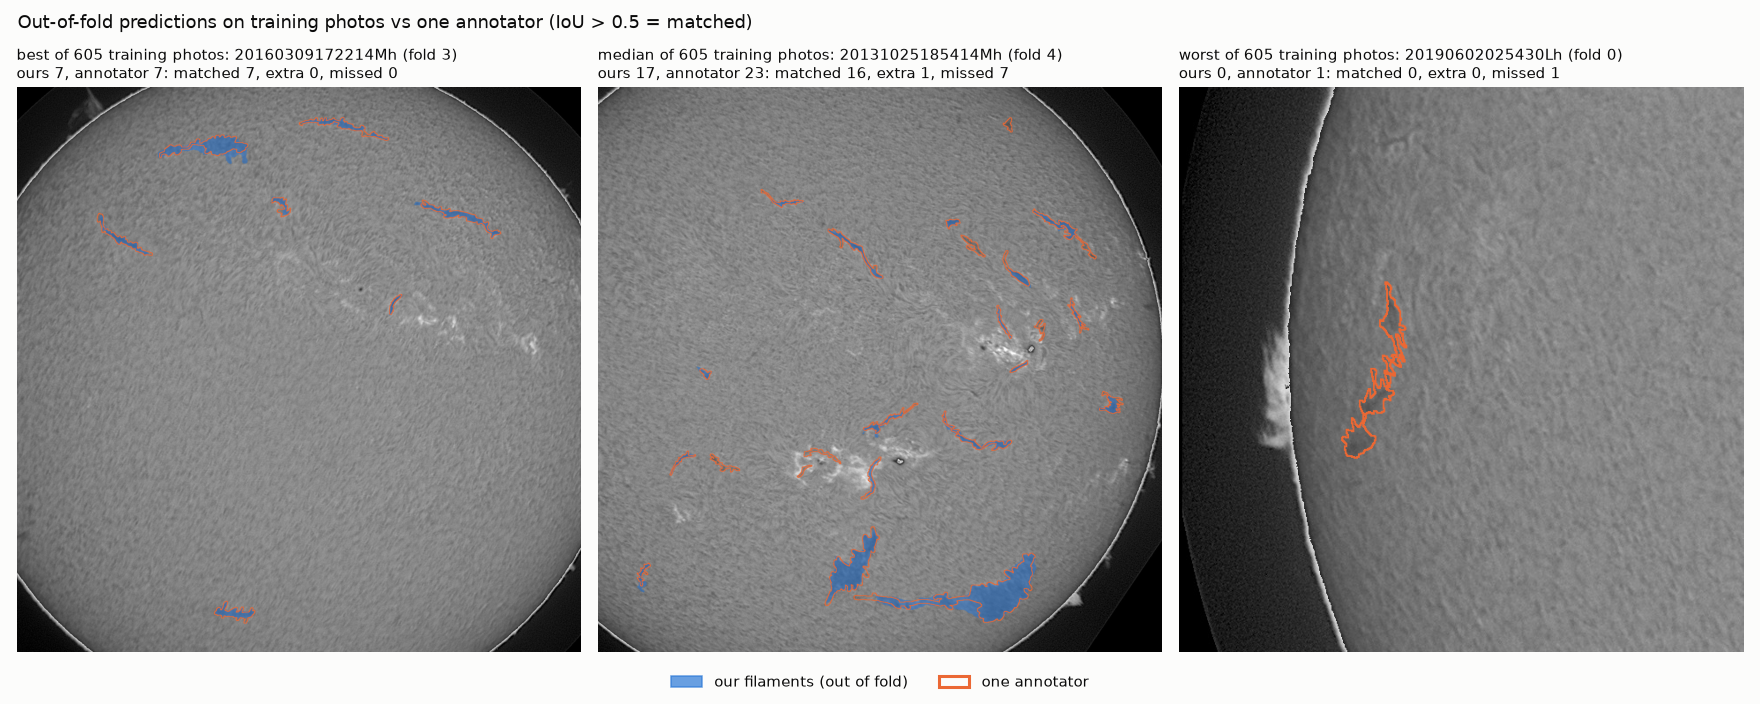
\includegraphics[width=0.64\textwidth]{figures/oof_predictions.png}
\caption{Out-of-fold predictions (filled blue) and one annotator's filaments (orange outlines) on three training observations, predicted by models and a scorer that never saw them: the best, the median and the worst observation by match rate.}
\label{fig:examples}
\Description{Three crops of solar disk images with predicted filaments filled in blue and one annotator's filaments outlined in orange.}
\end{figure*}

\chg{\begin{figure*}[t]
\centering
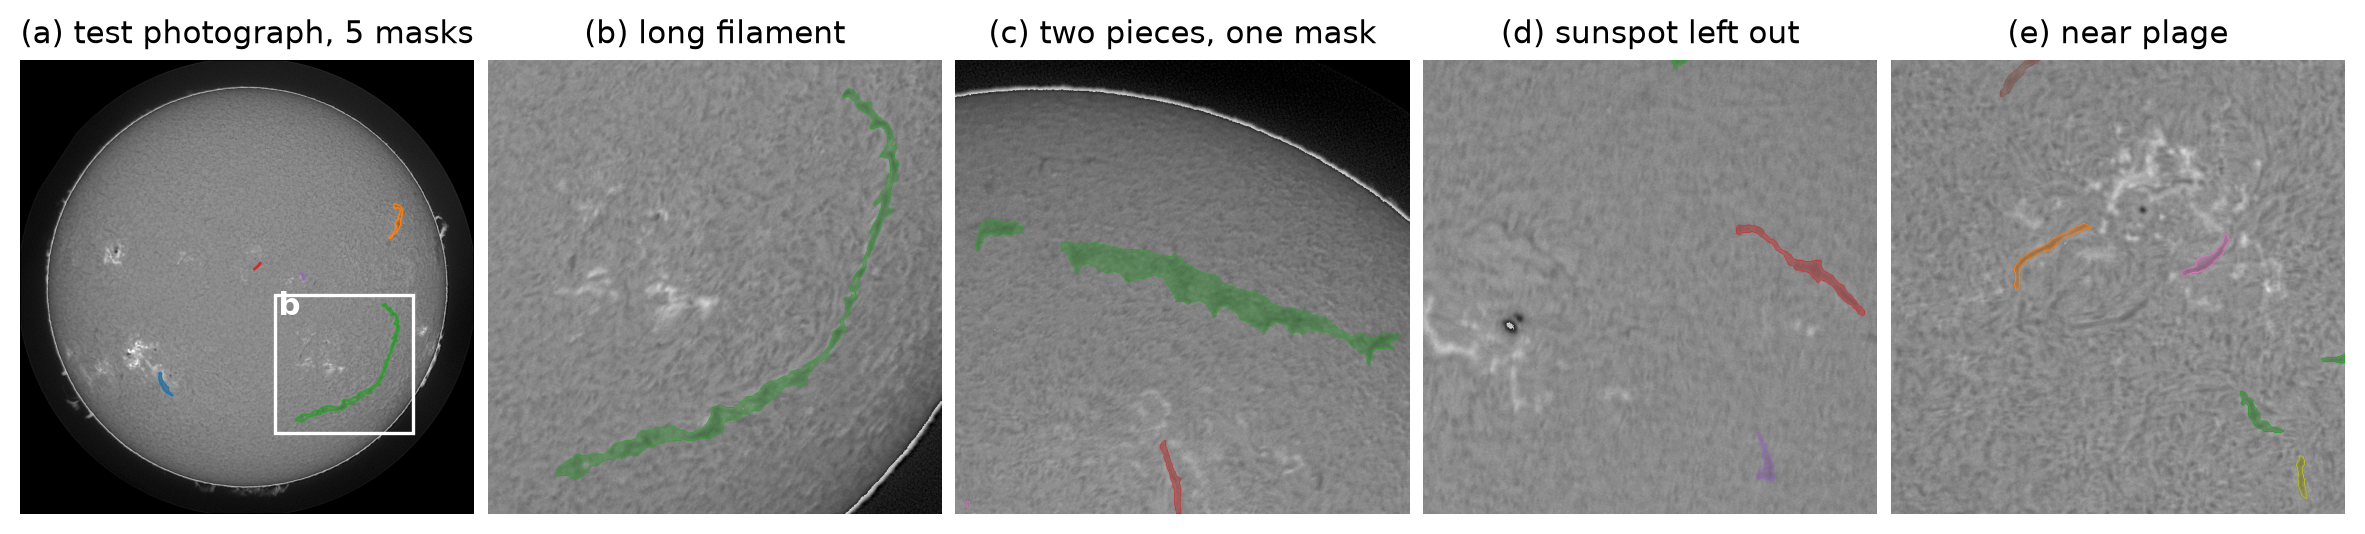
\includegraphics[width=\textwidth]{figures/morphology.png}
\caption{Submitted masks on H-$\alpha$ test photographs, one colour per mask: (a)~a full disk, whose sunspots and plage are not segmented; (b)~its long quiescent filament, kept as one thin mask that follows its curve; (c)~a broad filament in two pieces, submitted as one mask, as annotators often draw it; (d)~a sunspot left out, next to a filament; (e)~small filaments around an active region.}
\label{fig:morphology}
\Description{A full solar disk with five coloured filament masks, and four close-ups: a long curved filament, a broad filament in two pieces with one colour, a sunspot without mask next to a filament, and small filaments near a bright active region.}
\end{figure*}

\begin{table}[t]
\centering
\small
\caption{Shape of the 1,161 masks submitted on the 180 test photographs and of the 8,199 annotated training filaments: median [interquartile range]. Width: 4 times the mean distance to the background (the width of a uniform strip); elongation: area / width$^2$; solidity: area / convex-hull area; $R$: disk radius.}
\label{tab:morphology}
\setlength{\tabcolsep}{3.5pt}
\begin{tabular}{lcc}
\toprule
 & Submitted (test) & Annotated (train) \\
\midrule
Area (pixels) & 1270 [720, 2358] & 1228 [670, 2438] \\
Width (pixels) & 12.9 [10.7, 16.2] & 11.5 [9.3, 15.0] \\
Elongation & 7.7 [5.2, 10.9] & 9.0 [5.8, 13.9] \\
Solidity & 0.64 [0.49, 0.78] & 0.57 [0.44, 0.73] \\
In one connected piece & 90.4\% & 99.6\% \\
Centre beyond $0.9\,R$ & 0.2\% & 0.9\% \\
\bottomrule
\end{tabular}
\end{table}

\subsection{Morphology of the predicted segmentations}\label{sec:morphology}
PQ only counts matches above an IoU of 0.5, so we also look at the shape of the masks on the H-$\alpha$ photographs (Fig.~\ref{fig:examples} and~\ref{fig:morphology}) and compare their statistics with the annotations (Tab.~\ref{tab:morphology}, on different photographs, so only large differences matter). The masks are thin, elongated and often curved, like the filaments: median width 13 pixels, and three quarters are more than 5 times longer than wide. A long quiescent filament is kept as one mask along its whole curve (Fig.~\ref{fig:morphology}b), broad irregular filaments as broad masks (c), and small filaments are found next to active regions (e), while sunspots and the dark structures inside plage, as dark as filaments, are left out (a, d).

Three differences with the annotations stand out. (i)~The masks are slightly wider (12.9 against 11.5 pixels), less elongated (7.7 against 9.0) and more convex (solidity 0.64 against 0.57): their outlines are smoother and stop before the faint, thin ends that annotators include in their annotations. (ii)~One mask in ten has several separate pieces, against almost no annotation: some join the pieces of one filament across a gap, as annotators do (c), others are cut when masks are painted and lose pixels to a mask of higher $q$. (iii)~Faint filaments are missed, in particular near the limb, where foreshortening and limb darkening make them thinner and fainter: 0.2\% of the masks lie beyond $0.9\,R$, against 0.9\% of the annotations.


\gp{\subsection{Implementation details}\label{sec:details}
All models are trained with PyTorch in bf16 on 12\,GB GPUs. \textit{Mask2Former}: 50 epochs, AdamW with a learning rate of $10^{-4}$ ($10^{-5}$ for the backbone) and a cosine decay; a step holds 8 crops of 1024 pixels or, in a quarter of the steps, 2 whole photographs; the crops of the second family are zoomed by a random factor in $[0.8, 1.25]$. \textit{Candidates}: class probability at least 0.02, area at least 40 pixels, views linked at an IoU of 0.5. \textit{U-Nets}: inputs clipped to $[-6, 4]$. \textit{Scorer}: LightGBM with 300 rounds and 15 leaves, averaged over 10 seeds. \textit{Selection}: $\theta = 0.1$ and $\tau = 0.25$, from a grid on OOF PQ. \textit{Redraw}: $r = 2$ pixels, a shift of 0.25 pixel, and a minimum mask area of 100 pixels.}

% ==================================== %
%       CONCLUSION AND FUTURE WORK     %
% ==================================== %
\section{Conclusion and future work}\label{sec:conclusion}
We segmented solar filaments as instances by generating candidates with two Mask2Former families, scoring them with LightGBM and independent evidence models, selecting the best non-overlapping set exactly, and redrawing its boundaries at full resolution. It reaches an OOF PQ of 0.4801, above the 0.340 of inter-annotator agreement, and 0.42 / 0.39 on the public / private leaderboards.

The main limit is the annotations: on observations with several annotators, 71\% of the OOF misses of our first model were filaments that no other annotator drew, and 54\% of its false positives matched another annotator's filament. Our next steps are to train on the filaments that annotators agree on, and to learn when they join two pieces into one.}


% ==================================== %
%            ACKNOWLEDGMENT            %
% ==================================== %
\section{\texorpdfstring{\tpl{Acknowledgment}}{Acknowledgment}}\label{sec:acknowledgment}
    % Do not change
    \tpl{The organization of the Filament Segmentation Challenge 2026 is partially supported by the U.S. National Science Foundation (NSF) under Grant No. 2209912 and 2433781, directorate for Computer and Information Science and Engineering (CSE), and Office of Advanced Cyberinfrastructure (OAC), and Grant No. 2511630, AST Division Of Astronomical Sciences and MPS Directorate for Mathematical and Physical Sciences.}

    \tpl{The Filament Segmentation Challenge 2026 is sponsored by the U.S. National Science Foundation (NSF) National Solar Observatory (NSO).}

    \tpl{This work utilizes GONG data obtained by the NSO Integrated Synoptic Program, managed by the National Solar Observatory, which is operated by the Association of Universities for Research in Astronomy (AURA), Inc. under a cooperative agreement with the National Science Foundation and with contribution from the National Oceanic and Atmospheric Administration. The GONG network of instruments is hosted by the Big Bear Solar Observatory, High Altitude Observatory, Learmonth Solar Observatory, Udaipur Solar Observatory, Instituto de Astrofísica de Canarias, and Cerro Tololo Interamerican Observatory.}

\bibliographystyle{ACM-Reference-Format-citeorder}
\bibliography{main}

\end{document}
